%%%%%%%%%%%%%%%%%%%%%%%%%%%%%%%%%%%%%%%%%%%%%%%%%%%%%%%%%%%%%%%%%
% Contents : The accounts chapter
% $Id : grisbi-manuel-accounts.tex, v 0.4 2002/10/27 Daniel Cartron
% $Id : grisbi-manuel-accounts.tex, v 0.5.0 2004/06/01 Loic Breilloux
% some of its content was in tips chapter : 
% $Id : grisbi-manuel-tips.tex, v 0.4 2002/10/27 Daniel Cartron
% $Id : grisbi-manuel-accounts.tex, v 0.6.0 2011/11/17 Jean-Luc Duflot
% some of its content was in tips chapter :
% $Id : grisbi-manuel-tips.tex, v 0.5.0 2004/06/01 Loic Breilloux
% $Id : grisbi-manuel-accounts.tex, v 0.8.9 2012/04/27 Jean-Luc Duflot
% $Id : grisbi-manuel-accounts.tex, v 1.0 2014/02/12 Jean-Luc Duflot
% some of its content was in transactions chapter :
% $Id : grisbi-manuel-transactions.tex, v 0.8.9 2012/04/27 Jean-Luc Duflot
%%%%%%%%%%%%%%%%%%%%%%%%%%%%%%%%%%%%%%%%%%%%%%%%%%%%%%%%%%%%%%%%%

\chapter{Gestion des comptes\label{accounts} }

Grisbi sait gérer quatre types de compte, dont l'utilisation est décrite précisément dans la section \vref{accounts-type}, \menu{Types de compte de Grisbi} :
\begin{itemize}
	\item \indexword{compte bancaire}\index{compte !bancaire} : il permet de faire tout type d'opération ;
	\item \indexword{compte de caisse}\index{compte !caisse} : il ne permet de gérer que des espèces ;
	\item \indexword{compte de passif}\index{compte !passif} : il permet de gérer une dette que vous remboursez ; 
	\item \indexword{compte d'actif}\index{compte !actif} : il permet de gérer un bien qui se déprécie avec le temps. 
\end{itemize}


\section{Liste des comptes\label{accounts-list}}


Pour lister les comptes, déroulez d'abord l'onglet \menu{Comptes} dans le panneau de navigation en cliquant sur le petit triangle à sa gauche. Le panneau de navigation affiche la liste des comptes, que vous pouvez faire défiler en cliquant successivement sur l'un des deux petits triangles à gauche dans la barre d'information.

% espace avant Attention ou Note  : 5 mm
%\vspacepdf{5mm}
\textbf{Note} : ces triangles peuvent être remplacés, en fonction du thème de l'environnement de bureau ou du gestionnaire de fenêtres que vous utilisez, par d'autres caractères tels que +, -, >, <, etc.

% On pourrait dérouler la liste au clavier par la touche Espace, par exemple.

% espace pour changement de thème
\vspacepdf{5mm}
Vous pouvez modifier l'ordre d'affichage des comptes dans le panneau de navigation, en cliquant et déplaçant le nom d'un compte vers le haut ou vers le bas dans la liste des comptes du panneau de navigation.


\section{Sélection d'un compte\label{accounts-selection}}


Pour sélectionner et afficher le contenu d'un compte, utilisez l'une des méthodes suivantes :

\begin{itemize}
	 \item cliquez sur son nom dans le panneau de navigation ;
	 \item déplacez la sélection avec les touches  du clavier \key{Flèche Haut},  \key{Flèche Bas}, \key{Page Haut} ou \key{Page Bas}, ou avec la molette de la souris ;
	 \item dans la barre d'information, cliquez sur l'un des deux petits triangles à gauche pour faire défiler les comptes.
\end{itemize}

\textbf{Note} : ces triangles peuvent être remplacés, en fonction du thème de l'environnement de bureau ou du gestionnaire de fenêtres que vous utilisez, par d'autres caractères tels que +, -, >, <, etc.

% espace pour changement de thème
\vspacepdf{5mm}
Le panneau de navigation affiche le nom du compte sur fond bleu{\couleur} ; la barre d'information affiche, à gauche, le nom du compte sélectionné et, complètement à droite, le solde de ce compte ; le pavé des détails affiche la liste des opérations dans l'onglet \menu{Opérations}.

% espace pour changement de thème
\vspacepdf{5mm}
Le pavé des détails affiche par défaut deux onglets, pour les comptes de banque ou de caisse :
\begin{itemize}
	 \item l'onglet \menu{Opérations} ;
	 \item l'onglet \menu{Propriétés}.
\end{itemize}

Il peut aussi afficher, si le module budgétaire a été activé pour le compte sélectionné, trois autres onglets qui ne sont pas décrits dans ce chapitre (voir le chapitre \vref{budget}, \menu{Budgets Prévisionnels}) :
\begin{itemize}
	 \item soit les onglets \menu{Prévisions} et \menu{Données historiques}, pour les comptes de banque ou de caisse ;
	 \item soit l'onglet \menu{Tableau d'amortissement}, pour les comptes de passif.
\end{itemize}


% espace pour changement de thème
\vspacepdf{5mm}
Il se peut que certains comptes soient \indexword{clos}\index{compte !clos}, donc leur affichage est masqué. Vous pouvez cependant les afficher en sélectionnant le menu \menu{Affichage - Montrer les comptes clos}. Pour faire l'opération inverse, voir la section \vref{accounts-properties}, \menu{Propriétés d'un compte}. 


\section{Propriétés d'un compte\label{accounts-properties}}


L'onglet \menu{Propriétés} permet de renseigner et d'afficher les informations relatives au compte \ifIllustration sélectionné\refimage{account-new-properties-img}.
\else sélectionné.
\fi

\ifIllustration
% image centrée
\begin{figure}[h!]
\begin{center}
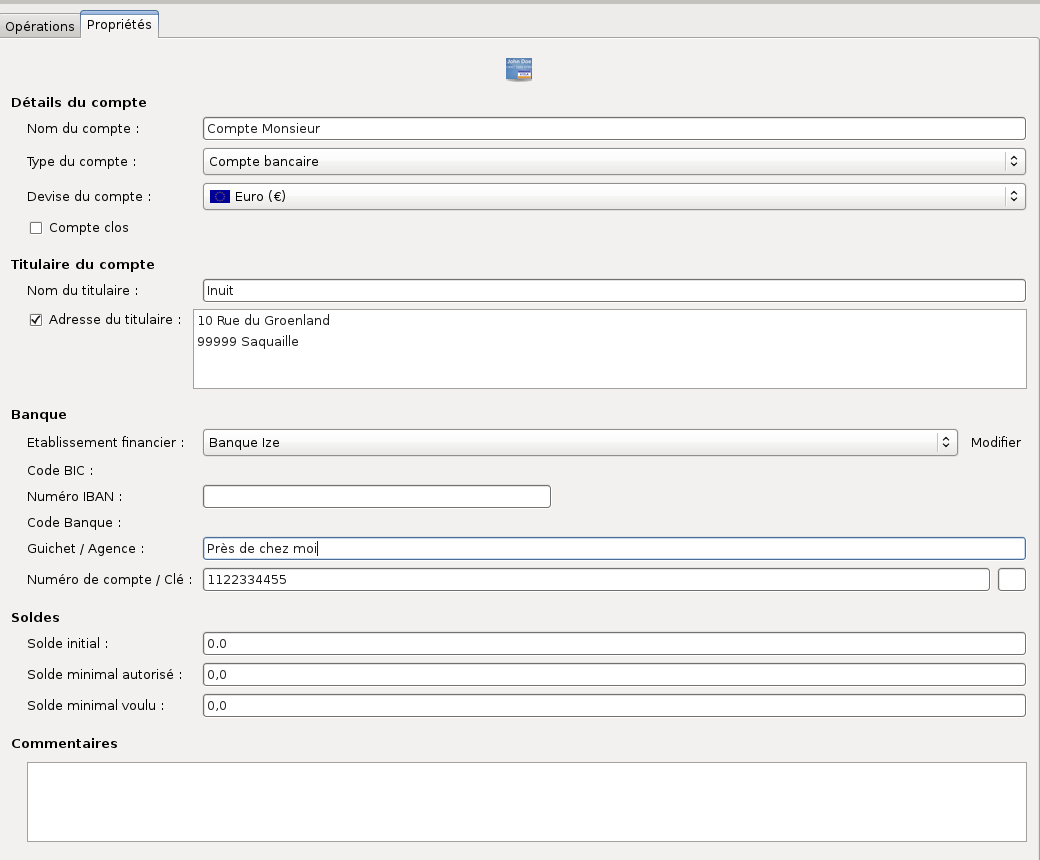
\includegraphics[scale=0.48]{image/screenshot/account_new_properties}
\end{center}
\caption{Propriétés d'un compte}
\label{account-new-properties-img}
\end{figure}
% image centrée
\fi

Pour afficher les propriétés d'un compte, sélectionnez-le, puis cliquez sur l'onglet \menu{Propriétés} dans le pavé des détails. Cet onglet affiche toutes les informations et propriétés qui ont déjà été renseignées sur le compte \ifIllustration sélectionné\refimage{account-new-properties-img}.
\else sélectionné.
\fi
Pour modifier ces données, voir la section \vref{accounts-modify}, \menu{Modifier un compte}.

Voici les différentes informations qu'un compte peut contenir :

\begin{itemize}
	\item \menu{Nom du compte} : ce peut-être un nom quelconque, par exemple \emph{Compte courant}, \emph{Compte livret}, \emph{Compte banque 1} ou \emph{Compte banque 2};	
% saut de ligne pour indentation correcte de la note dans la liste

\textbf{Note} : dans le cas d'une comptabilité numérotée (association ou petite entreprise), les noms des comptes sont précédés du numéro fourni par le plan comptable, par exemple \og 512. Compte banque X \fg{} ; ce libellé est donc une donnée alphanumérique.

	\item \menu{Type du compte} : pour plus de détails, voir la section \vref{accounts-type} ;	
	\item \menu{Devise du compte} : la devise dans laquelle les opérations de ce compte sont libellées (voir les sections \vref{setup-resources-currencies} et \vref{setup-resources-rate}) ;	
	\item \menu{{Compte clos}}\index{compte !clos} : case à cocher qui vous permet de masquer le compte dans le panneau de navigation et dans la barre d'information, sans pour autant le supprimer ; il pourra être affiché à nouveau en cliquant sur le menu \menu{Affichage - Montrer les comptes clos} ;	
	\item \menu{Nom du titulaire} : le titulaire d'un compte peut être différent pour chaque compte, par exemple si vous ouvrez un livret d'épargne pour chacun de vos enfants ;	
	 \item \menu{Adresse du titulaire} : le titulaire peut avoir la même adresse que le titulaire principal, ou bien une adresse différente qu'il faudra préciser ici (voir le paragraphe \vref{setup-display-addresses-address}, \menu{Adresses}) ;
	\item \menu{Établissement financier} : la banque qui gère votre compte ; vous pouvez choisir une banque indiquée dans la liste déroulante, ou bien cliquer sur \menu{Ajouter une nouvelle banque} ; il est conseillé de renseigner ce champ (voir la section \vref{setup-resources-banks}) ;	
	\item \menu{Numéro \gls{IBAN}} : le code que vous trouverez sur votre relevé d'identité bancaire (RIB) ou IBAN fourni par la banque (voir la section \vref{setup-resources-banks}) ;	
	\item \menu{Guichet / Agence} : l'adresse de votre agence bancaire, à relever également sur votre RIB (voir la section \vref{setup-resources-banks}) ;	
	\item \menu{Numéro du compte / Clé} : voir sur votre RIB (voir la section \vref{setup-resources-banks}) ;	
	\item \menu{Solde initial} : le solde de votre dernier relevé bancaire au moment de la création du compte ; il est conseillé de laisser le solde initial du compte à zéro et de créer par la suite une opération initiale du montant nécessaire, car cela facilitera la gestion future des rapprochements ;	
	\item \menu{Solde minimal autorisé} : le solde minimal que vous autorise votre
	établissement financier, plus communément appelé autorisation de découvert ;	
	\item \menu{Solde minimal voulu} : le solde minimal que vous aimeriez respecter ; pour un bon fonctionnement de la mise en couleur des soldes dans la page \menu{Accueil}, il doit être supérieur ou égal au solde minimal autorisé ;	
	\item \menu{Commentaires} : zone de saisie pour des commentaires informels sur le compte : date d'ouverture, taux de rendement, etc. (voir la section \vref{setup-resources-banks}).
\end{itemize}


\section{Création d'un nouveau compte\label{accounts-new}}


\textbf{Note} : avant de commencer la création d'un nouveau compte, il est conseillé de consulter la section \vref{accounts-type}, \menu{Types de compte de Grisbi}, et la section \vref{setup-resources-modes}, \menu{Modes de règlement}, qui donnent beaucoup plus de détails sur les possibilités que Grisbi vous propose.
% espace après Attention ou Note  : 5 mm
\vspacepdf{5mm}

Pour créer un nouveau compte dans votre fichier de comptes, cliquez sur le menu \menu{Édition - Nouveau compte} ; l'assistant de création de compte
s'ouvre, qui comprend cinq étapes :

\begin{enumerate}
	\item accueil de l'assistant ; validez par le bouton \menu{Suivant} ;
	\item sélection du type de compte : faites votre choix parmi les quatre types de compte proposés, puis validez par le bouton \menu{Suivant} ;
% espace pour Note ou Attention à la ligne dans une liste

\textbf{Note} : lorsque vous créez un nouveau compte, faites attention à choisir un type de compte correct, sinon vous pourriez être amené, plus tard, à transférer toutes les opérations que vous y auriez saisies dans un nouveau compte plus adéquat.
	\item créer un nouveau compte \ifIllustration \refimage{account-new-creation-img} :
	\else  :
	\fi
	
	\ifIllustration
	% image centrée
	\begin{figure}[htbp]
	\begin{center}
	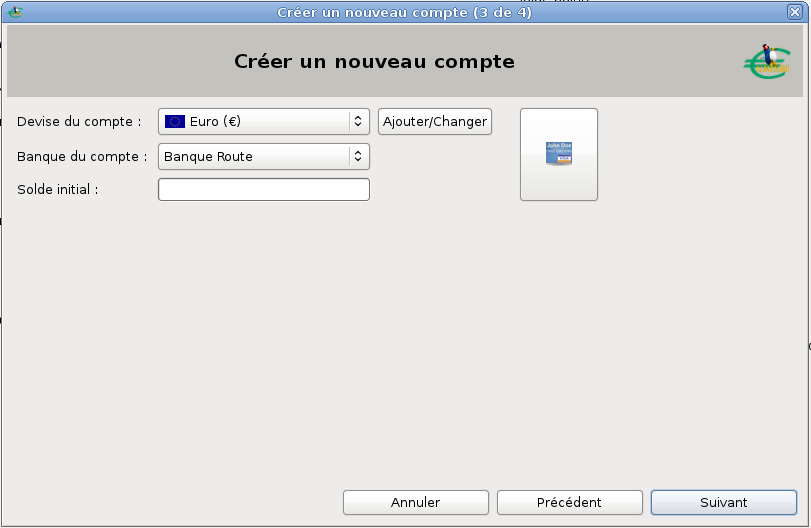
\includegraphics[scale=0.5]{image/screenshot/account_new_creation}
	\end{center}
	\caption{Création d'un nouveau compte}
	\label{account-new-creation-img}
	\end{figure}
	% image centrée
	\fi
	
		\begin{enumerate}
			\item choisissez la \indexword{devise}\index{devise} du compte dans la liste déroulante, qui propose les devises que connaît déjà votre fichier de comptes ; sinon, cliquez sur \menu{Ajouter/Changer}, une fenêtre s'affiche, où une liste déroulante vous propose toutes les devises du monde connues par Grisbi ; les détails de la devise sélectionnée s'affichent en-dessous, dans des champs que vous pouvez encore modifier ; puis validez par le bouton \menu{Fermer},
			\item choisissez la \indexword{banque}\index{banque !création} qui détient ce compte dans la liste déroulante, qui propose les banques que connaît déjà votre fichier de comptes ; sinon, cliquez sur \menu{Ajouter une nouvelle banque} : une fenêtre s'affiche, où vous pouvez renseigner le nom de la banque et de nombreux autres détails ; puis validez par le bouton \menu{Fermer},
			\item choisissez l'\indexword{icône}\index{icône} du compte : une fenêtre s'affiche, où vous pouvez soit choisir un répertoire dans la liste déroulante puis cliquer sur une des icônes en-dessous, soit chercher un fichier dans le système de fichiers de votre ordinateur (bouton \menu{Parcourir}) ; une fois votre icône trouvée, validez par le bouton \menu{Valider},
			\item saisissez le solde initial, puis validez par le bouton \menu{Suivant} ;
% espace pour Note ou Attention à la ligne dans une liste

\textbf{Note} : il est conseillé de laisser le solde initial du compte à zéro et, si besoin est, de créer par la suite une opération initiale du montant nécessaire, car cela facilitera la gestion future des rapprochements.
		\end{enumerate}

	\item saisissez le nom du \ifIllustration compte, celui qui apparaîtra dans le panneau de navigation, puis validez par le bouton \menu{Fermer}\refimage{account-new-name-img} ;
	\else compte, qui apparaîtra dans le panneau de navigation, puis validez par le bouton \menu{Fermer} ;
	\fi

	\ifIllustration
	% image centrée
	\begin{figure}[htbp]
	\begin{center}
	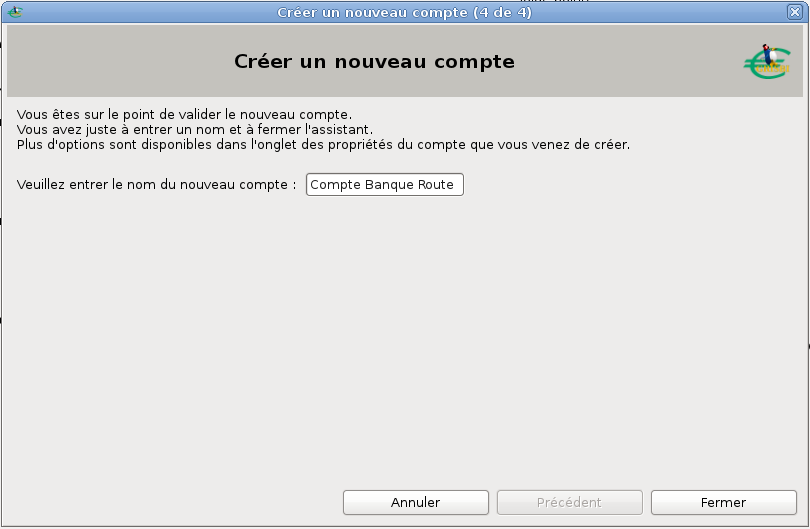
\includegraphics[scale=0.5]{image/screenshot/account_new_name}
	\end{center}
	\caption{Saisie du nom du nouveau compte}
	\label{account-new-name-img}
	\end{figure}
	% image centrée
	\fi
	\item le nouveau compte est alors créé, sélectionnez-le dans le panneau de navigation : son nom apparaît sur fond bleu{\couleur}, le pavé des détails affiche son onglet \menu{Opérations} qui est évidemment vide, et vous pouvez modifier ou compléter son onglet \menu{Propriétés}.
\end{enumerate}

%espace pour changement de thème
\vspacepdf{5mm}
Si, et seulement si vous venez de créer votre fichier de comptes juste avant cette création de compte, revenez à la fin de la section \vref{start-newfile-end}, \menu{Création d'un nouveau fichier de comptes}. Allez juste après la fin de la procédure de création du fichier de comptes, au paragraphe commençant par \emph{D'une manière ou d'une autre\ldots{ }}, ce qui vous proposera de créer tout de suite d'autres comptes.

%espace pour changement de thème
\vspacepdf{5mm}
Sinon, vous pouvez commencer à utiliser le compte que vous venez de créer.

%espace pour changement de thème
\vspacepdf{5mm}
Vous pouvez aussi configurer précisément les modes de règlement des opérations de ce compte dans le menu \menu{Édition - Préférences} (voir la section \vref{setup-resources-modes}, \menu{Modes de règlement}).


\section{Modification d'un compte\label{accounts-modify} }


Pour modifier un compte, sélectionnez le compte dans le panneau de navigation ou avec la barre d'information, puis cliquez sur l'onglet \menu{Propriétés} dans le pavé \ifIllustration des détails\refimage{account-new-properties-img}.
\else des détails.
\fi

Les champs suivants doivent obligatoirement être renseignés :
\begin{itemize}
	 \item le \menu{Nom du compte} ;
	 \item le \menu{Type du compte} ;
	 \item la \menu{Devise du compte} ;
	 \item le \menu{Solde initial}.
\end{itemize}
Tous les autres champs sont facultatifs. 


Vous pourrez modifier à tout moment \emph{toutes} ces informations, sauf la devise si vous avez choisi l'euro, ou si vous avez converti en euro un compte
existant, comme indiqué dans la section \vref{accounts-switcheuro}, \menu{Conversion d'un compte en euros}.

Les champs \menu{Type du compte}, \menu{Devise du compte}, \menu{Établissement financier} donnent accès à une liste déroulante permettant de renseigner le champ.

Les champs de texte peuvent être remplis au clavier, et un menu contextuel accessible par un clic-droit dans un champ de saisie permet d'effectuer les actions suivantes :
\begin{itemize}
	 \item \menu{Couper} (la sélection) ;
	 \item \menu{Copier} (la sélection) ;
	 \item \menu{Coller} (la sélection) ;
	 \item \menu{Supprimer} (la sélection) ;
	 \item \menu{Tout sélectionner} (dans le champ de saisie) ;
	 \item \menu{Méthodes de saisie} ;
	 \item \menu{Insérer un caractère de contrôle Unicode}\index{caractère de contrôle Unicode}.
\end{itemize}

%espace pour changement de thème
\vspacepdf{5mm}
Les \indexword{\gls{methodes de saisie}}\index{méthodes de saisie} permettent de changer les caractères accentués.

\indexword{Insérer un \gls{caractere de controle Unicode}} permet d'insérer un code Unichar qui modifie la présentation ; par exemple RLO (forçage droite-à-gauche) renverse l'ordre des lettres et la position du texte.

% espace avant Attention ou Note  : 5 mm
\vspacepdf{5mm}
\strong{Attention} : si vous modifiez certaines propriétés comme le type du compte, cela  nécessitera d'adapter aux nouvelles propriétés du compte, individuellement, toutes les opérations déjà saisies. Dans tous les cas, avant de procéder à une quelconque modification des comptes, faites \textbf{impérativement} une sauvegarde de votre fichier de comptes.

\ifIllustration
\else
% saut de page pour titre solidaire
\newpage
\fi

\section{Suppression d'un compte\label{accounts-delete} }


Pour supprimer un compte, cliquez sur le menu \menu{Édition - Supprimer le
compte courant}. Une boîte de dialogue de confirmation s'ouvre ; si
c'est vraiment ce que vous voulez, validez la suppression.

% espace avant Attention ou Note  : 5 mm
\vspacepdf{5mm}
\strong{Attention} : il n'y aura pas d'autre avertissement, et le compte est supprimé (ainsi que toutes ses opérations). Cette opération est \indexword{irréversible}\index{opération !irréversible} !


\section{Types de compte de Grisbi\label{accounts-type}}


Comme énoncé en début de chapitre, Grisbi sait gérer quatre \indexword{types de compte}\index{types de compte} :

\begin{itemize}
	\item compte bancaire : il permet de faire tout type d'opération ;
	\item compte de caisse : il ne permet de gérer que des espèces ;
	\item compte de passif : il permet de gérer une dette que vous remboursez ; 
	\item compte d'actif : il permet de gérer un bien qui se déprécie avec le temps. 
\end{itemize}

%espace pour changement de thème
\vspacepdf{5mm}
Cette section décrit les fonctionnalités et l'utilisation de chacun de ces types de compte.


\subsection{Type compte bancaire\label{accounts-type-bank}}

Le type de compte \emph{compte bancaire} admet tous les types d'opérations, en débit ou en crédit. De ce fait, il doit être utilisé pour tous les comptes suivants :
\begin{itemize}
	\item compte bancaire ou compte courant ;
	\item compte d'épargne ;
	\item compte de	\indexword{carte bancaire à débit immédiat}\index{carte bancaire !débit immédiat} ;
	\item compte de \indexword{carte de crédit}\index{carte bancaire !de crédit} ;		
	\item compte d'attente ;
	\item compte d'avances. 
\end{itemize}

Les paragraphes suivants décrivent ces comptes qui doivent utiliser le type de compte \emph{compte bancaire}.


\subsubsection{Compte bancaire, courant, d'épargne ou de carte bancaire à débit immédiat\label{accounts-type-bank-misc}}

Ces comptes servent à enregistrer toutes les opérations que vous pouvez faire avec votre banque : 

\begin{itemize}
	\item virement de compte à compte ;
	\item prélèvement sur le compte ;
	\item émission et dépôt de chèques ; 
	\item achat, remboursement, retrait et dépôt avec une \indexword{carte bancaire à débit immédiat}\index{carte bancaire !débit immédiat}. 
\end{itemize}


\subsubsection{Compte de carte de crédit\label{accounts-type-bank-creditcard}}

Un compte de carte de crédit est un compte de carte bancaire qui peut recevoir du débit, mais aussi du crédit, soit sous forme de virement, soit sous forme de prêt (par ex. un crédit renouvelable). Son solde peut donc être positif ou négatif.


\subsubsection{Compte d'attente\label{accounts-type-bank-waiting}}

Un compte d'attente sert à enregistrer des opérations (normalement des recettes) en attendant de les virer vers un compte bancaire ou de caisse. Il est normalement créditeur, jusqu'au moment du virement vers le compte bancaire ou de caisse, qui le ramène à un solde nul.

La \indexword{remise de chèques}\index{remise !chèques} et la \indexword{remise d'espèces}\index{remise !espèces} sont des exemples-type de l'utilité du compte d'attente. 
 
\paragraph{\textsl{Remise de chèques ou d'espèces  :}\label{accounts-type-bank-waiting-remittance}}

Si vous recevez peu ou peu souvent de chèques (ou d'espèces), le plus simple est de les saisir directement dans votre compte bancaire (ou dans votre compte de caisse). Dans ce cas, reportez-vous à la section \vref{transactions-new-cheque}, \menu{Remise de chèques ou d'espèces}.

% espace pour changement de thème
\vspacepdf{5mm}
Mais si vous recevez beaucoup de chèques (par exemple parce que vous gérez une association et que vos adhérents payent leur cotisation par chèque), le plus efficace est d'utiliser un compte d'attente.

% espace pour changement de thème
\vspacepdf{5mm}
La méthode consiste donc à créer un \emph{compte d'attente}, que vous nommez par exemple \emph{Chèques à encaisser}. Au fur et à mesure de la réception des chèques, vous les enregistrez individuellement dans ce compte, donc chaque chèque correspond à un \menu{Tiers}. Quand vous déposez les chèques à la banque, vous faites un virement de ce compte \emph{Chèques à encaisser} vers votre compte bancaire, du montant de l'ensemble de ces chèques, donc du solde du compte \emph{Chèques à encaisser}. Utilisez pour l'occasion un tiers \emph{Remise de chèques}, et dans le champ \menu{Remarques}, saisissez le numéro de votre bordereau de remise.
% (ce bordereau sera généré directement par Grisbi dans une prochaine version). 

Le solde du compte \emph{Chèques à encaisser} revient alors à zéro, et le compte bancaire est crédité du montant de la remise, exactement comme le sera votre relevé bancaire. Ainsi vous gardez et l'information du tiers pour chaque chèque, et celle de la remise globale.

Vous faites ensuite un pseudo-rapprochement du compte \emph{Chèques à encaisser} en simulant un relevé de solde nul avant la prochaine réception d'un chèque : vérifiez que ce rapprochement a bien un numéro, ou donnez-en lui un, par exemple REM-01, ce qui vous permettra ultérieurement de retrouver quel chèque faisait partie de quelle remise. Ce pseudo-rapprochement est appelé \emph{\indexword{lettrage}}\index{lettrage}.

% l'édition du bordereau de remise comportant \textbf{toutes} les opérations non-rapprochées (\emph{non fonctionnel pour l'instant, vous devrez créer ce bordereau à la main ou avec un logiciel de traitement de texte}).

%espace pour changement de thème
\vspacepdf{5mm}
Par exemple, si vous avez reçu deux chèques, vous enregistrez dans votre compte \emph{Chèques à encaisser} les deux opérations :

\begin{itemize}
	\item \menu{Date} : jj/mm/aa  \menu{Tiers} : Durand  \menu{Crédit} : 20  \menu{Catégorie} : \emph{Cotisations}  \menu{Mode de règlement} : \emph{Chèque}
	\item \menu{Date} : jj/mm/aa  \menu{Tiers} : Dupond  \menu{Crédit} : 40  \menu{Catégorie} : \emph{Cotisations}  \menu{Mode de règlement} : \emph{Chèque}
\end{itemize}

Puis lors de la remise des deux chèques à la banque, dans votre compte bancaire, vous enregistrez l'opération :

\begin{itemize}
	\item \menu{Date} : jj/mm/aa  \menu{Tiers} : Remise de chèques  \menu{Crédit} : 60  \menu{Catégorie} : \emph{Virement : Chèques à encaisser}  \menu{Mode de règlement} : \emph{Chèque}
\end{itemize}

\textbf{Note} : vous pouvez enregistrer cette opération soit dans votre compte bancaire en \menu{Crédit} et \menu{Catégorie} : \emph{Virement : Chèques à encaisser}, soit dans votre compte \emph{Chèques à encaisser} en \menu{Débit} et \menu{Catégorie} : \emph{Virement : Compte bancaire} ; dans les deux cas, Grisbi crée automatiquement la contre-opération dans l'autre compte.

Le compte \emph{Chèques à encaisser} est alors soldé à zéro, mais il garde la trace des chèques déposés à la banque, et dans votre compte bancaire n'apparaît que le montant global du bordereau de remise, que vous pourrez pointer avec votre relevé de compte de la banque.

%espace pour changement de thème
\vspacepdf{5mm}
Bien entendu, si une partie de vos adhérents vous paye en espèces, vous pouvez utiliser de la même façon un compte nommé par exemple \emph{Remise d'espèces}.


\subsubsection{Compte d'avances\label{accounts-type-bank-advance}}

Un compte d'avances sert à enregistrer à la fois les avances que vous recevez et celles que vous consentez. Il peut s'agir, par exemple, d'une avance sur votre salaire ou d'un achat que vous faites pour le compte d'un de vos amis.

% espace avant Attention ou Note  : 5 mm
\vspacepdf{5mm}
\textbf{Note} : le compte d'avances peut être déroutant pour le novice, puisqu'il fonctionne à l'envers, comme vous le découvrirez plus loin. Pour vous faciliter les choses, vous pouvez considérer que le compte d'avances se comporte comme un tiers qui vous donne ou à qui vous donnez de l'argent.

\paragraph{\textsl{Réception d'une avance  :}} quand vous \indexword{recevez une avance}\index{avance !réception}, vous enregistrez l'opération par un virement du compte d'avances vers un compte bancaire. Le tiers sera la personne ou l'organisation de qui vous recevez l'avance, et la catégorie sera \emph{Virement : Compte bancaire}. Dans le champ \menu{Notes}, vous indiquez le motif de l'avance. Le compte d'avances est donc débiteur quand vous devez de l'argent. Lorsque vous remboursez cette avance, vous faites un virement du compte bancaire, avec le même tiers et la même remarque, vers le compte d'avances, dont le solde redevient nul.

Pour une avance en espèces, remplacez le compte bancaire par un compte de caisse.

Dans le cas où l'avance vous est versée par chèque, et si vous avez créé un compte d'attente \emph{Chèques à encaisser}, vous devrez d'abord enregistrer le chèque dans le compte d'avances, puis faire un virement du montant du chèque, du compte d'avances vers ce compte \emph{Chèques à encaisser}, et ensuite faire votre virement de remise de chèque, de ce compte \emph{Chèques à encaisser} vers votre compte bancaire (voir le paragraphe \vref{accounts-type-bank-waiting}, \menu{Compte d'attente}). 

Vous ferez ensuite un rapprochement du compte d'avances pour faire disparaître ces opérations.

\paragraph{\textsl{Consentement d'une avance  :}} inversement, si vous \indexword{consentez une avance}\index{avance !consentement}, vous enregistrez l'opération par un virement d'un compte bancaire vers le compte d'avances. Le tiers sera la personne ou l'organisation à qui vous faites l'avance, et la catégorie sera \emph{Virement : Compte d'avances}. Dans le champ \menu{Remarques}, vous indiquerez le motif de l'avance. Le compte d'avances est donc créditeur quand on vous doit de l'argent. Lorsque cette avance vous est remboursée, vous enregistrez l'opération par un virement du compte d'avances vers le compte bancaire, avec le même tiers et la même remarque, et la catégorie sera \menu{Virement : Compte bancaire}. Le solde de votre compte d'avances redevient nul.

Pour une avance en espèces, remplacez le compte bancaire par un compte de caisse.

Dans le cas où l'avance vous est remboursée par chèque, et si vous avez créé un compte d'attente  \emph{Chèques à encaisser}, vous devrez d'abord enregistrer le chèque dans le compte d'avances, puis faire un virement du montant du chèque, du compte d'avances vers ce compte \emph{Chèques à encaisser}, et ensuite faire votre virement de remise de chèque, de ce compte \emph{Chèques à encaisser} vers votre compte bancaire  (voir le paragraphe \vref{accounts-type-bank-waiting}, \menu{Compte d'attente}). 

Vous ferez ensuite un rapprochement du compte d'avances pour faire disparaître ces opérations.

%espace pour changement de thème
\vspacepdf{5mm}
Un compte d'avances vous permet donc de vérifier facilement si vos créances ou vos dettes sont éteintes. Sans cette méthode cette vérification est difficile, sinon impossible.

% espace avant Attention ou Note  : 5 mm
\vspacepdf{5mm}
\textbf{Note} : lorsque vous faites un état des recettes et dépenses, ces opérations devraient être \emph{transparentes}, puisqu'elles s'annulent deux à deux quand chaque avance est remboursée. En pratique, lors de l'édition de ce genre d'état, vous devrez le configurer pour qu'il ne prenne pas en compte les virements entre comptes, et ainsi ces opérations seront totalement invisibles (voir la section \vref{reportscreation-selection-transfer}, \menu{Virements}).

% espace avant Attention ou Note  : 5 mm
\vspacepdf{5mm}
\textbf{Note} : lorsque vous créez un nouveau compte, choisissez donc de préférence le type de compte \emph{compte bancaire}, sauf si votre nouveau compte devra avoir une utilisation plus spécifique comme celles décrites dans les paragraphes ci-dessous.


\subsection{Type compte de caisse\label{accounts-type-cash}}

Le type de compte \emph{compte de caisse} est destiné uniquement aux opérations réglées en espèces ; vous ne pouvez pas y sélectionner de mode de paiement et il ne peut en aucun cas devenir négatif. De ce fait, il doit être utilisé pour tous les comptes suivants :
\begin{itemize}
	\item compte de caisse ;
	\item porte-monnaie électronique. 
\end{itemize}

% espace pour changement de thème  : 5 mm
\vspacepdf{5mm}
Un compte de caisse permet d'enregistrer dans votre comptabilité les retraits de la banque, pour alimenter la caisse, et les recettes et dépenses en espèces. En ce qui concerne les dépenses, il n’est pas toujours possible ni même utile d’enregistrer toutes les menues dépenses. Mais vous pouvez les enregistrer globalement, par exemple en fin de mois, dans des catégories adéquates ou bien dans une catégorie \menu{Dépenses diverses}, ceci afin de vider ce compte de caisse. Comme ceci, vous n’aurez pas de flou dans la caisse.

Un compte de caisse accepte les virements en provenance d'autres comptes. Lorsque vous faites un retrait en espèces sur votre compte bancaire, enregistrez-le en tant que virement vers le compte de caisse.


\subsection{Type compte de passif\label{accounts-type-liabilities}}

Le type de compte \emph{compte de passif} est un compte qui représente une dette, par exemple un \indexword{emprunt}\index{emprunt}. De ce fait, il doit être utilisé pour tous les comptes suivants :

\begin{itemize}
	\item compte d'emprunt ;
	\item compte de \indexword{carte bancaire à débit différé}\index{carte bancaire !débit différé}.
	
\end{itemize}


\subsubsection{Compte d'emprunt\label{accounts-type-liabilities-loan}}

Un compte d'emprunt sert à gérer un emprunt. Son solde initial est nul, mais, dès que vous contractez une dette, il devient négatif du montant de cette dette, et augmente ensuite à chaque remboursement versé, pour devenir nul après son dernier remboursement. 

En pratique, le solde initial de ce compte est nul, mais il devient (fortement) négatif dès la première opération, à savoir le virement, par l'organisme de crédit, du montant de l'emprunt sur votre compte courant. Vous enregistrez à ce moment-là un virement du compte de passif vers ce compte courant, ce qui vous permet de procéder à votre achat.

Par exemple, quand l'organisme de crédit Crédit Bitoire vous verse le montant de 20 000 pour acheter chez Auto Matique une voiture qui coûte 25 000, vous créez un compte de passif appelé \emph{Emprunt}, et dans ce compte, vous saisissez l'opération suivante : 

\begin{itemize}
	\item \menu{Date} : jj/mm/aa  \menu{Tiers} : Crédit Bitoire  \menu{Débit} : 20 000  \menu{Catégorie} : \emph{Virement : Banque Yze} \menu{Remarques} : Dette emprunt Crédit Bitoire
\end{itemize}

\textbf{Note} : si ce virement est fait directement par l'organisme de crédit sur le compte du vendeur, la catégorie devra être, par exemple, \emph{Virement : Compte Immobilisation}; vous pouvez n'avoir qu'un seul compte d'immobilisation pour tous vos biens, ou bien un compte par bien acheté.

%espace pour changement de thème
\vspacepdf{5mm}
À chaque fois que vous versez une échéance de votre \indexword{emprunt}\index{emprunt}, vous enregistrez un virement de votre compte courant vers le compte \emph{Emprunt}, du montant du capital remboursé, en catégorie \emph{Virement : Emprunt}, et une dépense sur ce compte courant, du montant des intérêts, en catégorie \emph{Frais financiers : Charges d'emprunts}. Éventuellement, ajoutez-y une dépense pour l'assurance, en catégorie \emph{Assurances}. De cette façon, vous saurez à tout moment le montant du capital restant à rembourser, mais aussi le coût de l'emprunt.

Par exemple, à chaque échéance, vous saisissez une opération ventilée sur votre compte courant :

\begin{itemize}
	\item opération maître  : \menu{Date} : jj/mm/aa  \menu{Tiers} : Crédit Bitoire  \menu{Débit} : 350  \menu{Catégorie} : \emph{Opération ventilée}
	\item 1\up{re} opération ventilée : \menu{Débit} : 300  \menu{Catégorie} : \emph{Virement : Emprunt}
	\item 2\up{e} opération ventilée : \menu{Débit} : 50  \menu{Catégorie} : \emph{Frais financiers : Charges d'emprunts}
\end{itemize}

%espace pour changement de thème
\vspacepdf{5mm}
N'oubliez pas que, si le montant de l'échéance est constant, à l'intérieur de chaque échéance suivante, le capital remboursé augmente et l'intérêt versé diminue (voir le tableau d'amortissement de l'emprunt).  

%espace pour changement de thème
\vspacepdf{5mm}
Vous pourrez donc parfaitement utiliser un compte de passif pour gérer vos emprunts ; comme Grisbi ne propose pas pour l'instant la ventilation automatique des remboursements d'emprunt (amortissements, intérêts et frais reportés automatiquement de votre tableau d'amortissement), vous pourrez tout de même saisir une opération planifiée et ventilée pour les remboursements, en mode manuel ou automatique, et vous ajusterez les montants à chaque échéance selon votre tableau (voir la section \vref{credit-amortization}, \menu{Tableau d'amortissement}).

%espace pour changement de thème
\vspacepdf{5mm}
Lorsqu'un compte de passif est soldé, ce qui signifie que vous avez remboursé la dette correspondante, Grisbi vous prévient en affichant un message dans la partie inférieure du pavé des détails de la page d'accueil (voir le chapitre \vref{home}, Accueil). 


\subsubsection{Compte de carte bancaire à débit différé\label{accounts-type-cash-deferredCards}}

Les cartes bancaires à débit différé peuvent être gérées de différentes manières, mais il est préférable de les gérer dans un compte spécifique, qui sera de type compte de passif, puisque leur solde ne peut pas être positif.

Vous trouverez tous les détails pour gérer correctement ces cartes bancaires dans la section \vref{bankcard-deferredCard}, \menu{Carte bancaire à débit différé}.


\subsection{Type compte d'actif\label{accounts-type-assets}}

Le type de compte \emph{compte d'actif} est un compte qui représente un bien, par exemple une voiture. Son solde initial est nul, mais il devient positif dès que vous possédez ce bien, d'un montant égal à sa valeur, puis il diminue avec le temps à mesure de sa dépréciation, pour finir à une valeur nulle. Les opérations se font par virement. On peut le considérer comme le  contraire d'un compte de passif.

%espace pour changement de thème
\vspacepdf{5mm}
En pratique, le solde initial de ce compte est nul, mais il devient (fortement) positif dès la première opération, à savoir l'achat de ce bien. Vous enregistrez à ce moment-là un virement de votre compte courant vers ce \indexword{compte d'actif}\index{actif !compte}, égal au prix d'achat du bien, ce qui vous permet de procéder à votre achat.

Par exemple, quand vous achetez la voiture à 25 000 chez Auto Matique, vous créez un compte d'actif appelé \emph{Compte Immobilisation}, et dans votre compte courant, vous saisissez l'opération suivante : 

\begin{itemize}
	\item \menu{Date} : jj/mm/aa  \menu{Tiers} : Auto Matique  \menu{Débit} : 25 000  \menu{Catégorie} : \menu{Virement : Compte Immobilisation}  \menu{Remarques} : Actif achat voiture
\end{itemize}

Votre compte \emph{Immobilisation} enregistre donc une opération en crédit, du montant de cette voiture.

%espace pour changement de thème
\vspacepdf{5mm}
À chaque fois que vous constatez une \indexword{dépréciation}\index{dépréciation !actif}\index{actif !dépréciation} de ce bien, vous enregistrez un retrait du compte d'actif, du montant de la dépréciation, dans la catégorie \emph{Amortissements : Dépréciation}. Ces retraits pourront être faits jusqu'à ce que le solde du compte soit nul. De cette façon vous connaîtrez en permanence la valeur de votre bien.

Par exemple, au bout d'un an la cotation de votre voiture (par ex. dans votre journal préféré) a perdu une certaine valeur ; dans votre compte \emph{Immobilisation}, vous saisissez l'opération suivante : 

\begin{itemize}
	\item \menu{Date} : 31/12/2012  \menu{Tiers} : Dépréciation Voiture  \menu{Débit} : 5000  \menu{Catégorie} : Amortissements : Dépréciation
\end{itemize}

%espace pour changement de thème
\vspacepdf{5mm}
Lors de l'achat, le montant que vous possédez réellement est votre apport personnel. Au cours du temps, vous remboursez les mensualités de votre emprunt, tandis que votre bien se déprécie. Le solde des comptes d'actif et de passif vous donnera à tout moment le montant que vous possédez globalement.


\section{Conversion d'un compte en euros\label{accounts-switcheuro}}


Cette section devient de plus en plus obsolète au fur et à mesure que le 
temps passe, mais nous la maintenons encore pour vous permettre l'éventuel
import de vieux fichiers de compte.

Cette fonction n'existe plus à partir de la version 0.8 de Grisbi. Donc, si vous avez absolument
besoin de réaliser cette opération, le seul moyen serait de la faire en utilisant une version précédente, de la manière suivante :

% espace avant Attention ou Note  : 5 mm
\vspacepdf{5mm}
\strong{Attention} : cette procédure n'est qu'une proposition, et n'a pas été
testée avec toutes les versions précédentes de Grisbi. C'est pour cela qu'il est
de la plus haute importance de sauvegarder auparavant votre fichier de comptes en lieu sûr.

\begin{enumerate}
	 \item avant tout, faites une copie de votre fichier de comptes actuel, renommez-le (par ex. en \file{comptesSauvegarde.gsb)} et placez-le en lieu sûr ;
	 \item choisissez une version ancienne de Grisbi, la moins ancienne possible 	et qui dispose de la fonction de conversion en euros ; vous devriez pouvoir la trouver, ainsi que son manuel, à la page du site de \lang{Grisbi}\footnote{\urlGrisbi{}} ; installez-la ;
	 \item importez le compte voulu en suivant les instructions du manuel de cette ancienne version de Grisbi que vous venez d'installer ;
	 \item procédez à la conversion de ce compte en euros ;
	 \item exportez ce compte en suivant les instructions du même manuel ; vous obtenez alors un fichier d'export ;
	 \item redémarrez votre nouvelle version de Grisbi et ouvrez votre fichier de comptes habituel (pas la sauvegarde, évidemment !) ;
	 \item procédez à l'importation du fichier d'export ;
	 \item si tout se passe bien, vous disposez maintenant de votre compte converti en euros.
\end{enumerate}

% espace avant Attention ou Note  : 5 mm
\vspacepdf{5mm}
\strong{Attention} : d'une manière générale, il est déconseillé d'avoir des accents ou des espaces dans les noms des répertoires et fichiers utilisés par Grisbi. Si c'est le cas, renommez-les maintenant. Par exemple, les espaces peuvent être remplacées par des tirets bas (\_). 

